\subsection{A Polynomial Time Algorithm For Solving \mainproblem}\label{sect:st-dPaths}

\begin{algorithm}[t]
\caption{Solving the \texttt{\mainproblem} problem.}\label{ALGO:solve}
\DontPrintSemicolon
\nonl \SetKwProg{Fn}{Procedure}{}{}
\footnotesize
\Fn{$\texttt{solve\_\mainproblem}(S, T, \nonviableset, n)$}{
\KwIn{an instance $\langle S, T, \nonviableset, n\rangle$ of \mainproblem.}
\KwOut{a pair $\langle \texttt{YES}, \p\rangle$ where the path $\p$ is
a solution to {\mainproblem} if such a path exists, \texttt{NO} otherwise.}
$d_{S,T}\leftarrow |T|-|S|$; \label{algo:solve:l1} \hfill\tcp{let $d_{S,T}$ be the distance between $S$ and $T$}
$\S \leftarrow \{S\}$; $\ell_\uparrow\leftarrow 0$; \label{algo:solve:l2}
                \tcp{init the \emph{frontier} $\S$ and its \emph{level counter} $\ell_\uparrow$ }
$\T \leftarrow \{T\}$; $\ell_\downarrow\leftarrow 0$; \label{algo:solve:l3}
                \tcp{init the \emph{frontier} $\T$ and its \emph{level counter} $\ell_\downarrow$ }
\While{\texttt{TRUE}}{ \label{algo:solve:l4}
    $\langle \S, \T, \ell_\uparrow, \ell_\downarrow \rangle\leftarrow
        \texttt{double-bfs\_phase}(\S, \T, \nonviableset, \ell_\uparrow, \ell_\downarrow, d_{S,T}, n)$; \label{algo:solve:l5} \;
    \If{ $\S=\emptyset$ \texttt{ OR } $\T=\emptyset$ \texttt{ OR }
                ($\ell_\uparrow + \ell_\downarrow = d_{S, T}$ \texttt{ AND } $\S\cap \T=\emptyset$)}{ \label{algo:solve:l6}
    \Return{\texttt{NO}}; \label{algo:solve:l7}
    }
    \If{ $\ell_\uparrow + \ell_\downarrow = d_{S,T}$ \texttt{ AND } $\S\cap\T\neq \emptyset$ }{ \label{algo:solve:l8}
        $\p\leftarrow\texttt{reconstruct\_path}(\S, \T, n)$; \label{algo:solve:l9} \;
        \Return{$\langle \texttt{YES}, \p \rangle$}; \label{algo:solve:l10}
    }
    $\texttt{returned\_val}\leftarrow\texttt{compression\_phase}(\S, \T, \nonviableset,
                            \ell_\uparrow, \ell_\downarrow, d_{S,T}, n)$; \label{algo:solve:l11} \;
    \lIf{$\texttt{returned\_val}=\langle \texttt{YES}, \p \rangle$}{\Return{$\p$};} \label{algo:solve:l12}
    \lElse{$\T\leftarrow \texttt{returned\_val}$;} \label{algo:solve:l13}
}
}
\end{algorithm}
We now describe a polynomial time algorithm for solving {\mainproblem}, called
\texttt{solve\_\mainproblem()}, which
takes as input an instance $\langle S, T, \nonviableset, n\rangle$ of \mainproblem, and
returns a pair $\langle \texttt{YES}, \p\rangle$ where $\p$ is a directed path in $\H_n$ that goes from source $S$ to target $T$
avoiding $\nonviableset$ if such a path exists (otherwise, the algorithm simply returns \texttt{NO}).
Algorithm~\ref{ALGO:solve} shows the pseudocode for that procedure.
The rationale at the base of \texttt{solve\_\mainproblem()} consists in the continuous iteration of two major phases:
\texttt{double-bfs\_phase()} (line~\ref{algo:solve:l5})
and
\texttt{compression\_ phase()} (line~\ref{algo:solve:l11}).
Throughout computation, both phases alternate repeatedly
until a final state of termination is eventually reached
(either at line~\ref{algo:solve:l7}, line~\ref{algo:solve:l10} or line~\ref{algo:solve:l12}).
At that point, the algorithm either returns a pair $\langle \texttt{YES},
\p \rangle$ where $\p$ is the sought directed path, or a negative response \texttt{NO} instead.
We now describe both phases in more detail, and give the corresponding pseudocode.

\paragraph{Breadth-First Search phases}
The first search $\texttt{BFS}_\uparrow$ starts from the source vertex $S$ and moves upward,
from lower to higher levels of $\H_n$.
Meanwhile, it collects a certain (polynomially bounded) amount of vertices that do not lie in $\nonviableset$.
In particular, at the end of any $\texttt{BFS}_\uparrow$ phase,
the number of collected vertices will always
lie between $|\nonviableset|\, d_{S,T} + 1$ and $|\nonviableset|\, d_{S,T}\,n$
(see line~\ref{algo:bfs:l1} of \texttt{bfs\_phase()}).
The set $\S$ of vertices collected at the end of $\texttt{BFS}_\uparrow$ is called the \emph{(source) frontier} of $\texttt{BFS}_\uparrow$.
All vertices within $\S$ have the same cardinality, \ie $|X_1|=|X_2|$ for every $X_1,X_2\in \S$.
Also, the procedure keeps track of the highest level of depth $\ell_\uparrow$ that is reached during $\texttt{BFS}_\uparrow$.
Thus, $\ell_\uparrow$ corresponds to the distance between the source vertex $S$ and
the current frontier $\S$,
formally, $\ell_\uparrow = |X|-|S|$ for every $X\in \S$.
Since at the beginning of the computation $\texttt{BFS}_\uparrow$ starts from the source vertex $S$,
\texttt{solve\_\mainproblem()} initializes $\S$ to $\{S\}$ and $\ell_\uparrow$ to $0$ at line~\ref{algo:solve:l2}.

\begin{algorithm}[t]
\caption{Breadth-First-Search phases.}\label{ALGO:double_bfs}
\DontPrintSemicolon
\SetKwProg{Fn}{Procedure}{}{}
\footnotesize
\nonl\Fn{\texttt{double-bfs\_phase}$(\S, \T, \nonviableset, \ell_\uparrow, \ell_\downarrow, d_{S,T}, n)$}{
\setcounter{AlgoLine}{0}

$\langle \S^*, \ell^*_\uparrow \rangle\leftarrow
	\texttt{bfs\_phase}(\S, \nonviableset, \ell_\uparrow, \ell_\downarrow,
		\texttt{out}, d_{S,T}, n)$; \label{algo:two_bfs:l1} \tcp{$\text{BFS}_\uparrow$}
$\langle \T^*, \ell^*_\downarrow \rangle\leftarrow
 \texttt{bfs\_phase}(\T, \nonviableset, \ell_\downarrow, \ell^*_\uparrow,
		\texttt{in}, d_{S,T}, n)$; \label{algo:two_bfs:l2} \tcp{$\text{BFS}_\downarrow$}
\Return{$\langle \S^*, \T^*, \ell^*_\uparrow, \ell^*_\downarrow \rangle$}; \label{algo:two_bfs:l3} \;
}

\SetKwProg{SubFn}{SubProcedure}{}{}
\nonl\SubFn{\texttt{\textbf{bfs\_phase}}$(\X, \nonviableset, \ell_x, \ell_y, \texttt{drt}, d_{S,T}, n)$}{
\setcounter{AlgoLine}{0}

\While{ $1\leq|\X|\leq |\nonviableset|\, d_{S,T} \texttt{ AND } \ell_x + \ell_y < d_{S,T} $ }{ \label{algo:bfs:l1}
	$\X\leftarrow \texttt{next\_step\_bfs}(\X, \nonviableset, \texttt{drt}, n)$; \label{algo:bfs:l2} \;
	$\ell_x\leftarrow \ell_x+1$; \label{algo:bfs:l3} \;
}
\Return{$\langle \X, \ell_x \rangle$}; \label{algo:bfs:l4}
}

\setcounter{AlgoLine}{0}

\nonl\SubFn{$\texttt{\textbf{next\_step\_bfs}}(\X, \nonviableset, \texttt{drt}, n)$}{
\setcounter{AlgoLine}{0}
$\X'\leftarrow\emptyset$; \label{algo:next_bfs:l1} \;
\ForEach{$v\in \X$}{ \label{algo:next_bfs:l2}
	$\X'\leftarrow \X'\cup N^{\texttt{drt}}(v)\setminus \nonviableset$;\hfill\tcp{$N^{\texttt{drt}}$ is $N^{\texttt{in}}$ if $\texttt{drt}=\texttt{in}$, otherwise it is $N^{\texttt{out}}$ \label{algo:next_bfs:l3}}
}
\Return{$\X'$}; \label{algo:next_bfs:l4}
}
\end{algorithm}

Similarly, the second search $\texttt{BFS}_\downarrow$ starts from the target vertex $T$ and moves downward,
from higher to lower levels of $\H_n$, also collecting a certain (polynomially bounded) amount of vertices that do not lie in $\nonviableset$.
As in the previous case, this amount will always
lie between $|\nonviableset|\, d_{S,T} + 1$ and $|\nonviableset|\, d_{S,T}\, n$.
The set $\T$ of vertices collected at the end of $\texttt{BFS}_\downarrow$
is called the \emph{(target) frontier} of $\texttt{BFS}_\downarrow$.
All vertices within $\T$ have the same cardinality.
Also, the procedure keeps track of the \emph{lowest} level of depth $\ell_\downarrow$ that $\texttt{BFS}_\downarrow$ has reached.
Thus, $\ell_\downarrow$ corresponds to the \emph{distance} between the target vertex $T$ and the frontier $\T$,
so that $\ell_{\downarrow}=|T|-|X|$ for every $X\in\T$. Since at the beginning of the computation,
$\texttt{BFS}_\downarrow$ starts from the target vertex $T$,
\texttt{solve\_\mainproblem()} initializes $\T=\{T\}$ and $\ell_\downarrow=0$ at line~\ref{algo:solve:l3}.
\figref{fig:double_bfs_phase} provides an illustration of the behaviour of \texttt{double-bfs\_phase()}.

In summary, after any round of \texttt{double-bfs\_phase()}, we are left with two (possibly empty) frontier sets $\S$ and $\T$.
In Algorithm~\ref{ALGO:solve}, whenever $\S=\emptyset$ or $\T=\emptyset$ holds at line~\ref{algo:solve:l6},
then at least one frontier set could not proceed one level further in $\H_n$ while avoiding $\nonviableset$,
and thus the procedure halts by returning \texttt{NO} at line~\ref{algo:solve:l7}.
Similarly, whenever $\ell_\uparrow+\ell_\downarrow = d_{S,T}$ and $\S\cap\T=\emptyset$ holds at line~\ref{algo:solve:l6},
the computation halts by returning \texttt{NO} at line~\ref{algo:solve:l7} --- the underlying intuition being that
$\S$ and $\T$ have finally reached one another's level of depth without intersecting each other,
which means that $\H_n$ contains no directed path from $S$ to $T$ that avoids $\nonviableset$.

\begin{figure}[htbp]
\centering
\begin{tikzpicture}[baseline= (a).base]
\node[scale=1] (a) at (0,0){
\begin{tikzcd}[
  every arrow/.append style={-,thick},
  matrix of math nodes maybe/.append style={/tikz/cells={/tikz/nodes={/tikz/draw,/tikz/shape=circle,align=center,text width=\widthof{$x_1x_2x_3$}}}},
  row sep=normal,
  column sep=large,
  thick,
  ]
        & 1,2,3 \dar \dlar \drar  \dar[shift left=.25cm, shorten=.1cm, -stealth]\\
\textit{\textbf{1,2}} & 1,3      \dlar \drar  & \textit{\textbf{2,3}} \\
 1 \uar
        &    \textit{\textbf{2}}         \ular \urar &   \textit{\textbf{3}} \uar\\
        & \emptyset \uar \ular \urar \ular[shift left=.25cm, shorten=.25cm, -stealth]
\end{tikzcd}
};
\end{tikzpicture}
\caption{A \texttt{double\_bfs\_phase()} on $\H_3$ that starts from $S=\emptyset$ and $T=\{1,2,3\}$.
The forbidden vertices are $\nonviableset=\{\{2\}, \{3\}, \{1,2\}, \{2, 3\}\}$,
 while the edges explored by $\texttt{BFS}_{\uparrow}$ and
$\texttt{BFS}_{\downarrow}$ are $(\emptyset, \{1\})$ and $(\{1,2,3\}, \{1,3\})$ (respectively).}\label{fig:double_bfs_phase}
\end{figure}

On the other
hand,
if both $\ell_\uparrow+\ell_\downarrow = d_{S,T}$ and
$\S\cap\T\neq\emptyset$ hold at line~\ref{algo:solve:l8},
then we can prove that for
every $S'\in\S$, there exists at least one directed path in $\H_n$
that goes from the source $S$ to $S'$ avoiding $\nonviableset$.
Similarly, for every $T'\in\T$, there exists at least one directed
path in $\H_n$ that goes from $T'$ to target $T$ avoiding $\nonviableset$.
Therefore, whenever $\S\cap\T\neq\emptyset$, the algorithm is in the right position to reconstruct
a directed path $\p$ in $\H_n$ that goes
from source $S$ to $\S\cap\T$ and from $\S\cap\T$ to target $T$ avoiding $\nonviableset$ (line~\ref{algo:solve:l9}).
In practice, the reconstruction can be implemented by maintaining a \texttt{map}
throughout the computation, which associates to every vertex $v$ (possibly visited during the BFSs)
the \emph{parent vertex}, $\texttt{parent}(v)$, which
led to discover $v$ first.
As soon as $\p$ gets constructed,
\texttt{solve\_\mainproblem()} returns $\langle\texttt{YES}, \p\rangle$
at line~\ref{algo:solve:l10},
and the computation halts.

\paragraph{Compression Phase}
After \texttt{double-bfs\_phase()} has completed,
the procedure \texttt{solve\_\mainproblem()} also needs to handle
the case
where $\S,\T\neq\emptyset$ and $\ell_\downarrow + \ell_\uparrow < d_{S,T}$.
The phase that starts at that point is named \texttt{compression\_phase()}
(see Algorithm~\ref{ALGO:compression_phase}).
\begin{algorithm}[t]
\caption{Compression phase.}\label{ALGO:compression_phase}
\nonl\SetKwProg{Fn}{Procedure}{}{}
\DontPrintSemicolon
\footnotesize
\Fn{$\texttt{\textbf{compression\_phase}}(\S, \T, \nonviableset, \ell_\uparrow, \ell_\downarrow, d_{S,T}, n)$}{
	$\T'\leftarrow\emptyset$; \label{algo:compression:l1} \;
	\While{\texttt{TRUE}}{ \label{algo:compression:l2}
		$\G\leftarrow\texttt{construct\_bipartite\_graph}(\S, \T, n)$; \label{algo:compression:l3}\;
		$\M\leftarrow\texttt{compute\_max\_matching}(\G, |\nonviableset|+1)$; \label{algo:compression:l4}\;
		\If{$|\M|>|\nonviableset|$}{ \label{algo:compression:l5}
    		  $\M_\S\leftarrow \{X\in\S\mid \exists\, Y\in \T\,\text{ s.t } ( X,Y ) \in \M\}$; \label{algo:compression:l6}\;
		  $\M_\T\leftarrow \{Y\in\T\mid \exists\, X\in \S\,\text{ s.t. } ( X,Y ) \in \M\}$; \label{algo:compression:l7}\;
		  $\{\p_1, \ldots, \p_{|\M|}\}\leftarrow
			\texttt{compute\_Lehman-Ron\_paths}(\M_\S, \M_\T, \M, n)$; \label{algo:compression:l8}\;
			$\p\leftarrow\texttt{reconstruct\_path}(\S, \T, \{\p_i\}_{i=1}^{|\M|}, n)$; \label{algo:compression:l9} \;
			\Return{$\langle \texttt{YES}, \p \rangle$}; \label{algo:compression:l10}
		}
		$\X\leftarrow \texttt{compute\_min\_vertex\_cover}(\G, \M)$; \label{algo:compression:l11}\;
		$\X_{\S}\leftarrow \X\cap \S$; $\X_\T\leftarrow \X\cap \T$; \label{algo:compression:l12}\;
		$\T'\leftarrow\T'\cup \X_\T$; \label{algo:compression:l13}\;
		$\langle \S, \T, \ell_\uparrow, \ell_\downarrow \rangle\leftarrow
			\texttt{double-bfs\_phase}(\X_\S, \T, \nonviableset,
				\ell_\uparrow, \ell_\downarrow, d_{S,T}, n)$; \label{algo:compression:l14} \;
		\If{ $\S=\emptyset$ \texttt{ OR } ($\ell_\downarrow + \ell_\uparrow = d_{S,T}$
						\texttt{ AND } $\S\cap \T=\emptyset$ )}{ \label{algo:compression:l15}
			\Return{$\T'$}; \label{algo:compression:l16}
		}
		\If{ $\ell_\uparrow + \ell_\downarrow = d_{S,T}$
				\texttt{ AND } $\S\cap\T\neq \emptyset$ }{ \label{algo:compression:l17}
			$\p\leftarrow\texttt{reconstruct\_path}(\S, \T, n)$; \label{algo:compression:l18} \;
			\Return{$\langle \texttt{YES}, \p \rangle$}; \label{algo:compression:l19}
		}
	}
}
\end{algorithm}
This procedure takes as input a tuple
$\langle \S, \T, \nonviableset, \ell_\uparrow, \ell_\downarrow, d_{S,T}, n \rangle$,
where $\S$ and $\T$ are the current frontier sets.
Recall that $|\T|>|\nonviableset|\, d_{S,T}$ holds due to line~\ref{algo:bfs:l1} of \texttt{bfs\_phase()}.
Also, $\nonviableset\subseteq\wp_n$ is the set of forbidden vertices;
$\ell_\uparrow$ is the level counter of $\S$ and $\ell_\downarrow$ is that
of $\T$; finally $d_{S,T}$ is the distance between the source $S$ and the target $T$, and $n$ is the size of the ground set.
The output returned by \texttt{compression\_phase()} is either a path $\p$ going from source $S$ to target $T$
avoiding $\nonviableset$ \texttt{or} a subset $\T'\subset \T$ such that the following two basic properties hold:


(1) $|\T'|\leq |\nonviableset|\, d_{S,T}$, and
(2) if $\p$ is any directed path in $\H_n$ going from
$\S$ to $\T$ avoiding $\nonviableset$, then $\p$ goes from $\S$ to $\T'$.


This frontier set $\T'$ is dubbed the \emph{compression} of $\T$. The underlying rationale goes as follows.
On one hand, because of (1), it is possible to keep the search going on by applying yet another round of \texttt{double-bfs\_phase()} on input $\S$ and $\T'$
(in fact, the size of $\T$ has been compressed down to $|\T'|\leq |\nonviableset|\, d_{S,T}$,
thus matching the threshold condition ``$|\X|\leq |\nonviableset|\, d_{S,T}$" checked at line~1 of \texttt{bfs\_phase()}).
On the other hand, because of (2), it is indeed sufficient to seek for a directed path in $\H_n$ that goes from $\S$ to $\T'$ avoiding $\nonviableset$,
namely, the search can actually forget about $\T\setminus \T'$ because it leads to a dead end.
\begin{figure}[!htb]
    \centering
    \begin{tikzpicture}[scale=.68, level distance=35pt,sibling distance=9pt]
    \Tree [. \framebox{$(\S, \T)$}
        \edge node[left, xshift=-1ex]{};
    [. \framebox{$(\X^{(1)}_{\S}, \T )$}
     \edge node[left,xshift=-1ex]{};
     [. \framebox{$(\S^{(1)}, \T)$}
        \edge node[left, xshift=-1ex]{};
        [. \framebox{$(\X^{(2)}_{\S}, \T)$}
            \edge node[]{};
            [. \framebox{$(\S^{(2)}, \T)$}
                \edge node[left, xshift=-1ex]{};
                [. \framebox{$(\X^{(3)}_{\S}, \T)$}
                    \edge node[left, xshift=-.25ex, yshift=1ex]{$\vdots$};
[. \framebox{$(\S^{(\max_i-1)}, \T)$}
                        \edge node[left, xshift=-1ex]{};
                            [. \framebox{$(\X^{(\max_i)}_{\S}, \T)$}
                            ]
                        \edge node[right, xshift=1ex]{};
                        [. \framebox{$(\S^{(\max_i-1)}, \X^{(\max_i)}_\T)$}
                        ]
                        ]
]
                \edge node[right, xshift=1ex]{};
                    [. \framebox{$(\S^{(2)}, \X^{(3)}_\T)$}
                    ]
            ]
        ]
        \edge node[right, xshift=1ex]{};
        [. \framebox{$(\S^{(1)}, \X^{(2)}_\T)$}
        ]
     ]
    ]
    \edge node[right, xshift=1ex]{};
    [. \framebox{$(\S, \X^{(1)}_\T)$} ]
    ]
    \end{tikzpicture}
    \caption{The frontier sets of the \texttt{compression\_phase()}.}
\label{fig:compression_phase}
\end{figure}
We now describe \texttt{compression\_phase()} in more details,
and give a graphical summary in \figref{fig:compression_phase}.
The procedure repeatedly builds an undirected bipartite graph
$\G=(V_\G, E_\G)$,
where $V_\G=\S\cup\T$ and
every vertex
$U\in\S$ is adjacent to a vertex $V\in\T$
if and only if $U\subset V$.
It then uses the procedure \texttt{compute\_max\_matching()} to find a matching
$\M$ of size $|\M|=\min(m^*, |\nonviableset|+1)$,
  where $m^*$ denotes the size of a maximum cardinality matching of $\G$.
Notice that the following holds due to line~\ref{algo:bfs:l1} of $\texttt{bfs\_phase()}$:
\[|V_\G| = |\S| + |\T| \leq 2\,|\F|\, d_{S,T}\, n,\]
thus, we have the following bound on the size of its edge set:
\[|E_\G| \leq |V_\G|^2 \leq 4\,|\F|^2\, d^2_{S,T}\, n^2. \]

\begin{algorithm}[t]
\caption{Self-Reduction for computing $\M$.}\label{ALGO:self_reduction}
\nonl\SetKwProg{Fn}{Procedure}{}{}
\DontPrintSemicolon
\footnotesize
\Fn{$\texttt{\textbf{self-reduction}}(\G,k)$}{
$\M\leftarrow \emptyset$;\label{algo:self-red:l1}\;
  \lIf{$k=0$}{
      \Return{$\M$;\label{algo:self-red:l2}}
    }
    $\hat{v}\leftarrow$ pick one vertex $\hat{v}\in V$ having maximum degree $\delta(\hat{v})$ in $\G$;\label{algo:self-red:l3}\;
    \If{$\delta(\hat{v})<k$\label{algo:self-red:l4}}{
      $\M\leftarrow$ compute a matching $\M$ of $\G$ s.t. $|\M| = \min(m^*, k)$, with the Hopcroft-Karp's algorithm~\cite{HK73};\label{algo:self-red:l5}\;
    }
    \If{$\delta(\hat{v})\geq k$\label{algo:self-red:l6}}{
      $\G'\leftarrow$ remove $\hat{v}$ from $\G$; and call the resulting graph $\G'$;\label{algo:self-red:l7}\;
      $\M'\leftarrow \texttt{self-reduction}(\G’, k-1)$;\label{algo:self-red:l8}\;
      $\M\leftarrow$ there must be at least one edge $\{u,\hat{v}\}\in E_\G$ such that $u$ is not matched in $\M’$,
      therefore, add $\{u,\hat{v}\}$ to $\M’$; and assign the resulting matching to $\M$;\label{algo:self-red:l9}\;
    }
    \Return{$\M$;\label{algo:self-red:l10}}
}
\end{algorithm}

The fact is that, given that we are content with a cardinality matching of size at most $k = |\nonviableset| + 1$,
it is worth applying the following recursive $\texttt{self-reduction}(\G,k)$ (Algorithm~\ref{ALGO:self_reduction}),
on input $(\G, |\nonviableset|+1)$, in order to shrink the upper bound on the size of $|E_\G|$ from $|V_\G|^2$ down to $|V_\G|\cdot |\nonviableset|$:
at line~\ref{algo:self-red:l1}, $\M\leftarrow\emptyset$ is initialized to the empty set. At line~\ref{algo:self-red:l2}, if $k=0$, the empty matching $\M=\emptyset$ is returned.
Then, at line~\ref{algo:self-red:l3}, let $\hat{v}\in V$ be some vertex having maximum degree $\delta(\hat{v})$ in $\G$.
If $\delta(\hat{v})<k$ at line~\ref{algo:self-red:l4}, the Hopcroft-Karp's algorithm~\cite{HK73} is invoked at line~\ref{algo:self-red:l5}
to compute a matching $\M$ of $\G$ such that $|\M| = \min(m^*, k)$, where $m^*$ is the maximum cardinality of any matching in $\G$.
In practice, this step can be implemented in the same manner as a maximum cardinality matching procedure,
\eg as Hopcroft-Karp's algorithm~\cite{HK73}, although with the following basic variation:
if the size of the augmenting matching $\M$ eventually reaches the cut-off value $k$,
then \texttt{compute\_max\_matching()}
returns $\M$ and halts (\ie even if $m^* > k$).
Otherwise, $\delta(\hat{v})\geq k$ holds at line~\ref{algo:self-red:l6}. So, at line~\ref{algo:self-red:l7},
let $\G'$ be the graph obtained from $\G$ by removing $\hat{v}$ and all of its adjacent edges;
next, it is invoked $\texttt{self-reduction}(\G’, k-1)$ at line~\ref{algo:self-red:l8}, recursively; and, then, the returned matching is assigned to $\M'$.
Since $\delta(\hat{v})\geq k$, there must be at least one edge $\{u,\hat{v}\}\in E_\G$ such that $u$ is not matched in $\M’$,
therefore, $\{u,\hat{v}\}$ is added to $\M’$; and the corresponding matching is assigned to $\M$, at line~\ref{algo:self-red:l9}.
Finally, $\M$ is returned at line~\ref{algo:self-red:l10}. In so doing, as shown in Lemma~\ref{lemma:complexity_compression_phase},
the complexity of $\texttt{compute\_max\_matching()}$, at line~\ref{algo:compression:l4} of $\texttt{compression\_phase()}$ (Algorithm~\ref{ALGO:compression_phase}),
is going to improve by a factor $n\cdot d_{S,T}$.

The course of the next actions depends on
$|\M|$:

\begin{enumerate}
\item
If $|\M| = |\nonviableset|+1$,
then the procedure relies on Theorem~\ref{thm:algo_lehmanron}
to compute a family $\p_1, \p_2, \ldots, \p_{|\M|}$ of $|\M|$
vertex-disjoint directed paths in $\H_n$ that go from $\S$ to $\T$.
In order to do that, the procedure considers the subset $\M_\S\subseteq\S$ (resp. $\M_\T\subseteq\T$) of all vertices in $\S$ (resp. in $\T$)
that are
incident
to some edge in $\M$ (lines~\ref{algo:compression:l6} and~\ref{algo:compression:l7}).
Notice that the matching $\M$ can be viewed as a bijection between $\M_\S$ and $\M_\T$.
Then, the algorithm underlying Theorem~\ref{thm:algo_lehmanron}
gets invoked on input $\langle \M_\S, \M_\T, \M, n \rangle$ (line~\ref{algo:compression:l8}).
Once all the Lehman-Ron paths $\p_1, \p_2, \ldots, \p_{|\M|}$ have been
found,
it is then possible to reconstruct the sought directed path $\p$ in $\H_n$ that goes from
source $S$ to target $T$  avoiding $\nonviableset$ (line~\ref{algo:compression:l9}).
In fact, since $|\M|>|\nonviableset|$ by hypothesis, and since $\p_1, \p_2, \ldots, \p_{|\M|}$
are distinct and pairwise vertex-disjoint,
there must exist at least one path $\p_i$ that goes from $\S$ to $\T$  avoiding $\nonviableset$.
It is therefore sufficient to find such a path $\p_i=v_0v_1\cdots v_k$ by direct inspection.
At that point, it is possible to reconstruct a path $\p$ going from $S$ to $v_0$ (because $v_0\in\S$),
as well as a path going from $v_k$ to $T$ (because $v_k\in\T$).
As already mentioned, in practice, the reconstruction can be implemented by maintaining a \texttt{map}
that associates to every vertex $v$ (eventually visited during the BFSs)
the parent vertex that had led to discover $v$ first.
Then, $\langle\texttt{YES},\p\rangle$ is returned at line~\ref{algo:compression:l10}.

\item
If $|\M|\leq |\nonviableset|$, then the \texttt{compression\_phase()}
aims to \emph{compress} the size of $\T$ down to $|\T'|\leq|\nonviableset|\, d_{S,T}$
as follows. Notice that in this case
$\M$ is a maximum cardinality matching of $\G$, because $|\M|\leq |\nonviableset|$.
So, the algorithm computes a minimum cardinality
vertex-cover $\X$ of $\G$ at line~\ref{algo:compression:l11},
whose size is $|\M|$ by K\"{o}nig's theorem~\cite{Diestel2005}.
The algorithm then proceeds at line~\ref{algo:compression:l12} by considering the set $\X_\S=\X\cap\S$ (resp. $\X_\T=\X\cap\T$)
of all vertices that lie both in the vertex-cover $\X$ and in the frontier set $\S$ (resp. $\T$).
Here, it is crucial to notice that both
$|\X_\S|\leq |\nonviableset|$ and $|\X_\T|\leq |\nonviableset|$ hold,
because $|\X|=|\M|\leq|\nonviableset|$.
The fact that, since $\X$ is a vertex-cover of $\G$,
any directed path in $\H_n$ that goes from $\S$ to $\T$ must go either from
$\X_\S$ to $\T$ or from $\S\setminus \X_\S$ to $\X_\T$ plays a pivotal role. Stated otherwise,
there exists no directed path in $\H_n$ that goes from $\S\setminus \X_\S$ to $\T\setminus \X_\T$,
simply because $\X$ is a vertex cover of $\G$.
At that point, the compression $\T'$ gets enriched with
$\X_\T$ at line~\ref{algo:compression:l13}.

Then, \texttt{compression\_phase()}
seeks a directed
path in $\H_n$ that eventually goes from $\X_S$ to $\T$.
This is done at line~\ref{algo:compression:l14} by running
\texttt{double-bfs\_phase()}
on $\langle \X_\S, \T, \nonviableset, \ell_\uparrow, \ell_\downarrow, d_{S,T}, n \rangle$.
Since $|\X_\S|\leq |\nonviableset|$, that execution results into an update of
both the frontier set $\S$ and of its level counter $\ell_\uparrow$.
Let $\S^{(i+1)}$ be the updated value of $\S$ and let $\ell^{(i+1)}_\uparrow$ be that of $\ell_\uparrow$.
Note that, since $|\T| > |\nonviableset|\, d_{S,T}$ holds as a pre-condition of \texttt{compression\_phase()},
neither $\T$ nor $\ell_\downarrow$ are ever updated at line~\ref{algo:compression:l14}.
Upon completion of this supplementary \texttt{double-bfs\_phase()},
if $\S^{(i+1)}=\emptyset$ or both
$\ell^{(i+1)}_\uparrow+\ell_\downarrow = d_{S,T}$ \emph{and}
$\S^{(i+1)}\cap\T=\emptyset$ at line~\ref{algo:compression:l15},
then $\T'$
is returned at line~\ref{algo:compression:l16} of \texttt{compression\_phase()}.

Otherwise, if $\ell^{(i+1)}_\uparrow + \ell_\downarrow = d_{S,T}$ \emph{and} $\S^{(i+1)}\cap\T\neq\emptyset$ at line~\ref{algo:compression:l17},
the sought directed path $\p$ in $\H_n$ that goes from source $S$ to target $T$ avoiding $\nonviableset$
can be reconstructed from $\S^{(i+1)}$ and $\T$ at line~\ref{algo:compression:l18},
so that \texttt{compression\_phase()} returns $\langle \texttt{YES}, \p \rangle$
and halts soon after at line \ref{algo:compression:l19}.

Otherwise, if $\S^{(i+1)}\neq\emptyset$ and $\ell^{(i+1)}_\uparrow + \ell_\downarrow < d_{S,T}$,
the next iteration will run on the novel frontier set $\S^{(i+1)}$ and its updated level counter $\ell^{(i+1)}_\uparrow$.
It is not difficult to prove that each iteration increases $\ell_\uparrow$ by at least one unit,
so that the \texttt{while-loop} at line~\ref{algo:compression:l2} of \texttt{compression\_phase()}
can be iterated at most $d_{S,T}$ times overall.
In particular, this fact implies that $|\T'|\leq |\nonviableset|\, d_{S,T}$
always holds at line~16 of \texttt{compression\_phase()}.
\end{enumerate}

\figref{fig:compression_phase} illustrates the family of all frontier sets considered throughout \texttt{com\-pres\-sion\_phase()},
where the following notation is assumed:
$\max_i$ is the total number of iterations of the \texttt{while-loop}
at line~\ref{algo:compression:l2} of \texttt{compression\_phase()},
$\X^{(i)}$ is the vertex-cover computed at the $i^{\mbox{\tiny th}}$ iteration of line~\ref{algo:compression:l11},
$\X_\S^{(i)}$ and $\X_\T^{(i)}$ are the sets computed at the $i^{\mbox{\tiny th}}$ iteration of line~\ref{algo:compression:l12}, and
$\S^{(i)}$ is the frontier set computed at the $i^{\mbox{\tiny th}}$ iteration of line~\ref{algo:compression:l14}.
The compression of $\T$ (possibly returned at line~16)
is
$\T'=\bigcup_{i=1}^{\max_i} \X^{(i)}_\T$.


\subsection{A Remark On Decision Versus Search}\label{sect:remark_dec_search}

\Cref{ALGO:solve}
tackles
the \textsc{Search-Task} of \mainproblem.
If
we merely want to answer the \textsc{Decision-Task} instead,
we can simplify the algorithm
by immediately returning \texttt{YES} if $|\M|>|\nonviableset|$ at line~\ref{algo:compression:l5} of \texttt{compression\_phase()}.
This is because in that case,
Theorem~\ref{thm:LehmanRon} guarantees the existence of a family of
$|\M|>|\nonviableset|$ vertex-disjoint paths in $\H_n$
that go from the current source frontier $\S$ to the target frontier $\T$,
which suffices to conclude that at least one of those paths avoids $\nonviableset$.
This simplification
improves the time complexity of our algorithm for solving the \textsc{Decision-Task} by a polynomial factor
over that for the \textsc{Search-Task}.

\subsection{Correctness Analysis of Algorithm~\ref{ALGO:solve}}\label{subsect:correctness}
The present subsection aims to show that the procedure \texttt{solve\_\mainproblem()} is correct.
A formal statement of that is provided in the next theorem.

\begin{theorem}\label{thm:correctness_main}
Let $\mathcal{I}=\langle S, T, \F, n\rangle$ be any instance of \mainproblem.
Given $\mathcal{I}$ as input, the procedure \texttt{solve\_\mainproblem()} halts within a finite number of steps.
Moreover, it returns as output a directed path $\p$ in $\H_n$ that goes from source $S$ to target $T$ avoiding $\F$,
provided that at least one such path exists; otherwise, the output is simply \texttt{NO}.
\end{theorem}

We are going to show a sequence of results that shall ultimately lead us to prove \Cref{thm:correctness_main}.
Hereafter, it is assumed that $\langle S, T, \F, n\rangle$ is an instance
(of \mainproblem) given as input to the \texttt{solve\_\mainproblem()} procedure. \Cref{lemma:halt_double-bfs,lemma:pre_halt_compression,lemma:halt_compression} below show that procedures \texttt{double-bfs\_phase()} and \texttt{compression\_phase()}, which are called by \texttt{solve\_\mainproblem()}, halt within a finite number of steps.

\begin{lemma}\label{lemma:halt_double-bfs}
Any invocation of \texttt{double-bfs\_phase()} halts within a finite number of steps.
In particular, the \texttt{while-loop} at line~\ref{algo:bfs:l1}
of the \texttt{bfs\_phase()} iterates at most $d_{S,T}$ times.
\end{lemma}
\begin{proof}
Consider the \texttt{while-loop} at line~\ref{algo:bfs:l1} of \texttt{bfs\_phase()}.
At each iteration of line~\ref{algo:bfs:l3}, the level counter $\ell_x$ gets incremented.
Notice that this is the only line at which $\ell_x$ may be modified,
and also notice that $\ell_y$ is never modified. Therefore, $\ell_x+\ell_y$ can only increase and not decrease.
Since the \texttt{while-loop} at line~\ref{algo:bfs:l1} of \texttt{bfs\_phase()} halts as soon as $\ell_x+\ell_y=d_{S,T}$,
the thesis follows.
\end{proof}

\begin{lemma}\label{lemma:pre_halt_compression}
Each iteration of the \texttt{while-loop} at line~\ref{algo:compression:l2} of \texttt{compression\_phase()} increases
$\ell_\uparrow + \ell_\downarrow$ by at least one unit,
either until $\ell_\uparrow + \ell_\downarrow=d_{S,T}$ or until the procedure halts by reaching either
line~\ref{algo:compression:l10}, line~\ref{algo:compression:l16} or line~\ref{algo:compression:l19}.
\end{lemma}
\begin{proof} Consider any iteration of the \texttt{while-loop}
at line~\ref{algo:compression:l2} of \texttt{compression\_} \texttt{phase()}.
Let $\G$ be the bipartite graph computed at line~\ref{algo:compression:l3},
and let $\M$ be the matching of $\G$ computed at line~\ref{algo:compression:l4}.
If $|\M| > |\F|$, then line~\ref{algo:compression:l10} gets executed, so the procedure halts
within a finite number of steps by virtue of our discussion in \Cref{sect:VertexDisjointPaths}.
Otherwise $|\M|\leq |\F|$. Recall that, since $|\M|\leq |\F|$, then $\M$ is a maximum matching of $\G$;
also recall that $\X_\S = \X\cap\S$ where $\X$ is a minimum vertex cover of $\G$ (line~\ref{algo:compression:l12}).
Since $|\X|=|\M|$, then $|\X_\S|\leq|\X|=|\M|\leq|\F|$.
Moreover, since $|\M| \leq |\F|$, \texttt{double-bfs\_phase()} gets invoked
at line~\ref{algo:compression:l14} on input $\langle \X_\S, \T, \F, \ell_\downarrow, \ell_\uparrow, d_{S,T}, n \rangle$
and
halts within a finite number of steps by \Cref{lemma:halt_double-bfs}.
Let us analyze its behavior with respect to $\X_\S$.
If $\X_\S=\emptyset$, then \texttt{double-bfs\_phase()} returns an empty frontier set $\S$ as output,
which leads to the termination of \texttt{compression\_phase()} at line~\ref{algo:compression:l16}.
Moreover, if $\ell_\uparrow + \ell_\downarrow=d_{S,T}$,
then
\texttt{compression\_phase()} halts
either at line~\ref{algo:compression:l16} or at line~\ref{algo:compression:l19}.
Otherwise, we must have $1 \leq |\X_\S|\leq |\F|$ and $\ell_\uparrow+\ell_\downarrow < d_{S,T}$,
in that case the condition for entering the
\texttt{while-loop} at line~\ref{algo:bfs:l1} of the \texttt{bfs\_phase()} is satisfied;
therefore, at line~\ref{algo:bfs:l3} of \texttt{bfs\_phase()}, the level counter $\ell_\uparrow$
gets incremented.
This implies the thesis.
\end{proof}

\begin{lemma}\label{lemma:halt_compression}
Any invocation of \texttt{compression\_phase()} halts within a finite number of steps.
In particular, the \texttt{while-loop} at line~\ref{algo:compression:l2}
of the \texttt{compression\_phase()} iterates at most $d_{S,T}$ times.
\end{lemma}
\begin{proof}
Firstly, recall Lemma~\ref{lemma:pre_halt_compression}.
Then, notice that as soon as $\ell_\uparrow + \ell_\downarrow=d_{S,T}$
the \texttt{compression\_phase()}
then halts either at line~\ref{algo:compression:l16} (if $\S\cap\T=\emptyset$)
or at line~\ref{algo:compression:l19} (if $\S\cap\T\neq\emptyset$).
This implies that the \texttt{while-loop} at
line~\ref{algo:compression:l2} of \texttt{compression\_phase()}
iterates at most $d_{S,T}$ times.
\end{proof}

We now prove some useful properties of \texttt{compression\_phase()} and \texttt{solve\_\mainproblem()}.

\begin{lemma}\label{lemma:reconstruct_path}
The following invariant is maintained at each line of \texttt{solve\_\mainproblem()}
and at each line of \texttt{compression\_phase()}.
For every $S'\in\S$ there exists a directed path in $\H_n$ that goes from $S$ to $S'$ avoiding $\F$;
similarly, for every $T'\in\T$ there is a directed path in $\H_n$ that goes from $T'$ to $T$ avoiding $\F$.
\end{lemma}
\begin{proof}
At the beginning of the procedure $\S=\{S\}$ and $\T=\{T\}$, so the thesis holds.
At each subsequent step, the only way in which a novel vertex can be added either to $\S$ or $\T$
is by invoking the \texttt{double\_bfs\_phase()},
which preserves connectivity and avoids $\F$ by construction at line~\ref{algo:next_bfs:l3} of \texttt{next\_step\_bfs()}.
\end{proof}

\begin{lemma}\label{lemma:compression_path}
Assume that any invocation of \texttt{compression\_phase()} halts by returning $\langle\texttt{YES},\p\rangle$.
Then $\p$ is a directed path in $\H_n$ that goes from source $S$ to target $T$ avoiding $\F$.
\end{lemma}
\begin{proof}
If \texttt{compression\_phase()} returns $\p$ as output, then the last iteration of the
\texttt{while-loop} at line~\ref{algo:compression:l2} must reach
either line~\ref{algo:compression:l10} or line~\ref{algo:compression:l19}:
\begin{enumerate}
\item
Assume that line~\ref{algo:compression:l10} is reached at the last iteration.
Then, during that iteration, the matching $\M$ (computed at line~\ref{algo:compression:l4} on input $\G$) has size $|\M| > |\F|$.
Recall that $\G$ is a bipartite graph on bipartition $(\S, \T)$.
Let $\M_\S$ (resp. $\M_\T$ be the subset of all vertices in $\S$ (resp. $\T$) that
belong
to some edge in $\M$. Then, by Theorem~\ref{thm:LehmanRon}, there exist $|\M|$ vertex-disjoint directed paths in $\H_n$, say
$\p_1, \p_2, \ldots, \p_{|\M|}$, whose union contains all the vertices in $\M_\S$ and $\M_\T$.
Since $|\M|>|\F|$, at least one of those paths --- say, $\p_i=v_0\cdots v_k$ --- must avoid $\F$.
By Proposition~\ref{lemma:reconstruct_path}, the procedure
\texttt{reconstruct\_path()} (invoked at line~\ref{algo:compression:l9}) is
able
to compute a directed path $\p_{S, v_0}$ in $\H_n$ that goes from $S$ to $v_0$ avoiding $\F$
(because $v_0\in\S$, being the first step of $\p_i$), and it is also
able
to compute a directed path $\p_{v_k,T}$
that goes from $v_k$ to $T$ avoiding $\F$ (because $v_k\in\T$, being the last step of $\p_i$).
Let $\p=\p_{S, v_0} \p_i \p_{v_k,T}$ be the directed path obtained by concatenation.
\texttt{compression\_phase()} then returns $\p$ at line~\ref{algo:compression:l10}.
\item
Assume that line~\ref{algo:compression:l19} is reached at the last iteration.
Then, at that iteration, the condition checked at line~\ref{algo:compression:l17} of \texttt{compression\_phase()} must be satisfied;
that is, we have $\ell_\uparrow + \ell_\downarrow=d_{S,T}$ and $\S\cap\T\neq\emptyset$.
Let $X$ be an arbitrary vertex in $\S\cap\T$.
By \Cref{lemma:reconstruct_path}, there exists at least one directed path $\p_{S,X}$ in $\H_n$
that goes from $S$ to $X$ avoiding $\F$ (because $X\in\S$);
similarly, there exists at least one directed path $p_{X,T}$ in $\H_n$ that goes from $X$ to $T$ avoiding $\F$ (because $X\in\T$).
Therefore, during that iteration, the procedure \texttt{reconstruct\_path()}
(invoked at line~\ref{algo:compression:l18}) is
able
to compute a path $\p=\p_{S,X}\p_{X,T}$ that goes from $S$ to $X$, and then from $X$ to $T$, which is the result
returned by \texttt{compression\_phase()} at line~\ref{algo:compression:l19}.
\end{enumerate}
\end{proof}

The following result shows two useful properties of the frontier set returned by \texttt{compression\_phase()}, for which we will need additional notation.
Denote by $\max_i$ be the number of times that the \texttt{while-loop}
at line~\ref{algo:compression:l2} gets iterated throughout
the whole execution of the \texttt{compression\_phase()}.


Also, let us introduce the following notation, for each index $i\in [\max_i]$:
\begin{itemize}
\item let $\X^{(i)}$ be the vertex cover that is computed during the $i$-th iteration of line~\ref{algo:compression:l11};
\item let $\X_\S^{(i)}$ and $\X_\T^{(i)}$ be the sets computed during the $i$-th iteration of line~\ref{algo:compression:l12};
\item let $\S^{(i)}$ be the novel frontier set that is computed during the $i$-th iteration of line~\ref{algo:compression:l14};
\end{itemize}
Moreover, we assume the notation $\S^{(0)}=\S$,
so that $\X_\S^{(i)}=\S^{(i-1)}\cap \X^{(i)}$ holds for each iteration $i\in [\max_i]$.
Notice that, since $|\T| > |\F|\, d_{S,T}$ holds by hypothesis,
then $\T$ is not modified, at line~\ref{algo:compression:l14}, by the invocation of \texttt{double-bfs\_phase()}.
Indeed, $\T$ is never modified throughout the \texttt{compression\_phase()}.
Nevertheless, a novel set $\T'\subset\T$ gets constructed and possibly returned.


\begin{proposition}\label{prop:compressed_frontier}
Assume that the procedure \texttt{compression\_phase()} is invoked on input
$\langle \S, \T, \F, \ell_\uparrow, \ell_\downarrow, d_{S,T}, n \rangle$,
where $|\T| > |\F|\, d_{S,T}$ is required to hold as a pre-condition.
Also, assume that the procedure halts at line~\ref{algo:compression:l16}, returning a novel frontier set $\T'\subset \T$.
Then, the following properties hold:
\begin{enumerate}
\item $|\T'|\leq |\F|\, d_{S,T}$;
\item if $\p$ is any directed path  in $\H_n$ that goes from $\S$ to $\T$ avoiding $\F$, then $\p$ goes from $\S$ to $\T'$.
\end{enumerate}
\end{proposition}
\begin{proof}
Firstly notice that, if an invocation of the \texttt{compression\_phase()}
halts at line~\ref{algo:compression:l16} by returning a novel frontier set $\T'\subset \T$,
this means that neither line~\ref{algo:compression:l10} nor
line~\ref{algo:compression:l19} are ever reached throughout that invocation.
In particular this implies that, at each iteration $i$ of
the \texttt{while-loop} at line~\ref{algo:compression:l2},
the maximum matching $\M^{(i)}$ (computed at line~\ref{algo:compression:l4})
has size $|\M^{(i)}|\leq |\F|$; this fact is assumed throughout the whole proof.

\begin{enumerate}
    \item \emph{Proof of (1).} At each iteration $i\in[\max_i]$, the minimum vertex cover $\X^{(i)}$ has size:
\[|\X^{(i)}|=|\M^{(i)}|\leq |\F|.\]
Since $\X^{(i)}_\T=\X^{(i)}\cap\T$ at line~\ref{algo:compression:l12}, then $|\X^{(i)}_\T| \leq |\X^{(i)}| \leq |\F|$.
Moreover, recall that $\T'$ gets enriched by $\X^{(i)}$ at each iteration of line~\ref{algo:compression:l13},
so that the following holds at the termination of the \texttt{compression\_phase()}:
\[\T'=\bigcup_{i=1}^{\max_i} \X^{(i)}_\T.\] Also recall that, by Lemma~\ref{lemma:halt_compression},
the \texttt{while-loop} at line~\ref{algo:compression:l2} can be iterated at most $d_{S,T}$ times, so that $\max_i\leq d_{S,T}$.
Therefore, when \texttt{compression\_phase()} terminates, we have $|\T'|\leq |\F|\, d_{S,T}$.


\item \emph{Proof of (2).} In order to prove (2),
we exhibit a number of invariants which hold for each iteration of the \texttt{while-loop} at line~\ref{algo:compression:l2} of \texttt{compression\_phase()}.
In what follows, we assume that the procedure \texttt{compression\_phase()} gets invoked on input
$\langle \S,\T,\F,\ell_\uparrow, \ell_\downarrow, d_{S,T}, n \rangle$,
and that $\S^{(0)}=\S$ holds by notational convention.

\begin{itemize}
\item[] \begin{lemma}\label{lemma:inv:1}
Let $i\in[\max_i]$ be any iteration of the \texttt{while-loop} at line~\ref{algo:compression:l2} of \texttt{compression\_phase()}.
Let $\p$ be any directed path in $\H_n$ that goes from $\S^{(i-1)}$ to $\T$.
Then $\p$ goes either from $\X^{(i)}_\S$ to $\T$ or from $\S^{(i-1)}\setminus \X^{(i)}_\S$ to $\X^{(i)}_\T$.
In other words, there exists no directed path in $\H_n$ that
goes from $\S^{(i-1)}\setminus \X^{(i)}_\S$ to $\T\setminus \X^{(i)}_\T$.
\end{lemma}
\begin{proof}
Recall that $\X^{(i)}$ is a vertex cover of the bipartite graph defined as $\G^{(i)}=((\S^{(i-1)}, \T), \subset)$,
which is constructed during the $i$-th iteration of line~\ref{algo:compression:l3} within the procedure \texttt{compression\_phase()}.
Also, $\X^{(i)}_\S = \X^{(i)}\cap \S^{(i-1)}$ and $\X^{(i)}_\T = \X^{(i)}\cap \T$,
so that the existence of any directed path in $\H_n$ going from $\S^{(i-1)}\setminus \X^{(i)}_\S$ to $\T\setminus \X^{(i)}_\T$
would imply the existence of some edge of $\G^{(i)}$ that would be uncovered by $\X^{(i)}$,
contradicting the fact that $\X^{(i)}$ is vertex cover of $\G^{(i)}$.
\end{proof}

\figref{fig:undirected_bipartite_vertex_cover} illustrates the intuition underlying Lemma~\ref{lemma:inv:1}.

\begin{figure}[!htb]
    \centering
    \begin{tikzpicture}[scale=.8,transform shape,>=stealth]
    \node[circle, fill=black!30, draw] (t1) {$t_1$};
    \node[circle, draw, scale=1.5] (t1_cover) {};
    \node[circle, fill=black!30, xshift=1ex, draw, right = of t1] (t2) {$t_2$};
    \node[circle, fill=black!30, xshift=1ex, draw, right = of t2] (t3) {$t_3$};
    \node[circle, xshift=1.75ex, draw, scale=1.5, right = of t2] (t3_cover) {};
    \node[circle, fill=black!30, xshift=1ex, draw, right = of t3] (t4) {$t_4$};
    \node[circle, xshift=1.75ex, draw, right = of t3, scale=1.5] (t4_cover) {};
    \node[circle, fill=black!30, xshift=1ex, draw, right = of t4] (t5) {$t_5$};

    \node[circle, draw, below = of t1, yshift=-10ex] (s1) {$s_1$};
    \node[circle, draw, xshift=1ex, right = of s1] (s2) {$s_2$};
    \node[circle, draw, xshift=1.72ex, right = of s1, scale=1.5] (s2_cover) {};
    \node[circle, draw, xshift=1ex, right = of s2] (s3) {$s_3$};
    \node[circle, draw, xshift=1ex, right = of s3] (s4) {$s_4$};
    \node[circle, draw, xshift=1.72ex, right = of s3, scale=1.5] (s4_cover) {};
    \node[circle, draw, xshift=1ex, right = of s4] (s5) {$s_5$};
    \node[circle, draw, xshift=1.72ex, right = of s4, scale=1.5] (s5_cover) {};

    \node[circle, draw, below = of s3, yshift=-12ex] (bot) {$\bf{0}$};
    \node[circle, draw, above = of t3, yshift=12ex] (top) {$[\bf{n}]$};

    \node[left = of t1, xshift=4ex] (Tlbl) {$\T$};
    \node[left = of s1, xshift=6ex] (Slbl) {$\S^{(i-1)}$};
    \node[left = of Tlbl, xshift=7ex, yshift=6ex] (Glbl) {$\G^{(i)}$};

    \node[above = of t2, xshift=-2ex, yshift=3.5ex] (Hn) {$\H_n$};

    \node[circle, draw, above = of bot, xshift=-1ex, yshift=-2ex] (f1) {\tiny $\bf F$};
    \node[circle, draw, above = of bot, xshift=-9ex, yshift=1ex] (f2) {\tiny $\bf F$};
    \node[circle, draw, above = of bot, xshift=8.25ex, yshift=1.5ex] (f3) {\tiny $\bf F$};

    \node[circle, draw, below = of top, xshift=-1ex, yshift=3ex] (f4) {\tiny $\bf F$};
    \node[circle, draw, below = of top, xshift=-9ex, yshift=1ex] (f5) {\tiny $\bf F$};
    \node[circle, draw, below = of top, xshift=8ex, yshift=1.5ex] (f6) {\tiny $\bf F$};

    \draw[thick] (s1) edge [] (t1); \draw[thick] (s1) edge [] (t3);
    \draw[thick] (s2) edge [] (t2); \draw[thick] (s2) edge [] (t5);
    \draw[thick] (s3) edge [] (t3); \draw[thick] (s3) edge [] (t4);
    \draw[thick] (s4) edge [] (t2); \draw[thick] (s4) edge [] (t5);
    \draw[thick] (s5) edge [] (t2); \draw[thick] (s5) edge [] (t5);

    \draw[dashed, ultra thin, rounded corners=15pt] (-2,.75) rectangle (8.2,-4); \draw[dashed, ultra thin, rounded corners=15pt] (-1.5,.65) rectangle (8,-.65); \draw[dashed, ultra thin, rounded corners=15pt] (-1.75,-2.65) rectangle (8,-3.9); 

    \draw[dashed, thick] (bot.west) edge [] (s1.south west);
    \draw[dashed, thick] (bot.east) edge [] (s5.south east);
    \draw[dashed, thick] (top.west) edge [] (t1.north west);
    \draw[dashed, thick] (top.east) edge [] (t5.north east);

    \draw[->, dotted, thick]  plot[smooth, tension=.7] coordinates {(3.4,-6.1) (2.8,-5.5) (2.5,-5) (1.75,-4.7) (1.5,-4) (.3,-3.5)};
    \draw[->, dotted, thick]  plot[smooth, tension=.7] coordinates {(3.58,-6) (3,-5.5) (3,-5) (3.15,-4.7) (3,-4) (2.23,-3.4)};
    \draw[->, dotted, thick]  plot[smooth, tension=.7] coordinates {(3.8,-6.1) (4,-5.5) (4.2,-5) (4.2,-4.7) (3.75,-4) (3.64,-3.4)};
    \draw[->, dotted, thick]  plot[smooth, tension=.7] coordinates {(4,-6) (4.5,-5.5) (4.45,-5) (4.35,-4.7) (4.45,-4) (5.4,-3.43)};
    \draw[->, dotted, thick]  plot[smooth, tension=.7] coordinates {(3.9,-6.1) (4.7,-5.5) (4.8,-5) (5.4,-4.7) (6.15,-4) (6.8,-3.3)};

    \draw[<-, dotted, thick]  plot[smooth, tension=.7] coordinates {(3.3,2.95) (2.4,2.5) (2.1,2) (1.75,1.7) (1.25,0.8) (.26,0.25)};
    \draw[<-, dotted, thick]  plot[smooth, tension=.7] coordinates {(3.58,2.9) (3.2,2.5) (3,2) (3.15,1.7) (3,0.8) (2.17,0.25)};
    \draw[<-, dotted, thick]  plot[smooth, tension=.7] coordinates {(3.8,2.9) (3.9,2.3) (3.9,2) (4,1.7) (3.75,0.8) (3.64,.35)};
    \draw[<-, dotted, thick]  plot[smooth, tension=.7] coordinates {(4,3.1) (4.35,2.2) (4.35,2) (4.4,1.7) (4.67,.6) (5.4,0.33)};
    \draw[<-, dotted, thick]  plot[smooth, tension=.7] coordinates {(4.15,3.1) (4.5,2.5) (5.25,2) (5.5,1.7) (6.5,.6) (7.35,0.35)};
    \end{tikzpicture}
    \caption{The undirected bipartite graph $\G^{(i)}=((\S^{(i-1)},\T), \subset)$, 
	and vertex cover $\X^{(i)}=(X^{(i)}_\S, X^{(i)}_\T)$ (doubly-circular nodes).}
\label{fig:undirected_bipartite_vertex_cover}
\end{figure}

\item[] \begin{lemma}\label{lemma:inv:2}
Let $i\in[\max_i]$ be any iteration of the \texttt{while-loop} at line~\ref{algo:compression:l2} of \texttt{compression\_phase()}.
Let $U$ be any subset of $\S^{(i-1)}$ and let $V$ be any subset of $\T$. Let $\p$ be any directed path in $\H_n$ that goes from $U$ to $V$.
Then $\p$ goes from $\S$ to $V$ in $\H_n$.
\end{lemma}
\begin{proof}
Induction on $i\in[\max_i]$.
\begin{itemize}
\item \emph{Base Case.} If $i=1$, recall that $\S^{(0)}=\S$. Then $U\subseteq \S$, which  implies the base case.
\item \emph{Inductive Step.}
Let us assume, by induction hypothesis, that the claim holds for some $i\in[\max_i-1]$
and let us prove it for $i+1$.
So, let $U\subseteq \S^{(i)}$, and let $\p$ by any directed path
in $\H_n$ that goes from $U$ to $V$.
Recall that $\S^{(i)}$ is the frontier set that
is returned by an invocation of \texttt{double-bfs\_phase()}
on input $\X^{(i)}_\S$, at the $i$-th iteration of line~\ref{algo:compression:l14}, within \texttt{compression\_phase()}.
This amounts to saying that all vertices in $\S^{(i)}$ have been discovered by a BFS starting from $\X^{(i)}_\S$.
Recall that $\X_\S^{(i)}=\X^{(i)}\cap\S^{(i-1)}$ so that $\X_\S^{(i)}\subseteq \S^{(i-1)}$.
Therefore, $\p$ is indeed a directed path in $\H_n$ that goes from $\S^{(i-1)}$ to $V$ in $\H_n$.
By induction hypothesis, the thesis follows.
\end{itemize}
\end{proof}

\item[] \begin{lemma}\label{lemma:inv:3}
Let $i\in[\max_i]$ be any index of iteration of the \texttt{while-loop}
at line~\ref{algo:compression:l2} of \texttt{compression\_phase()}.
Let $\p$ be a directed path in $\H_n$ that goes from $\S$ to $\T$  avoiding $\F$.
Then, $\p$ goes either from $\X^{(i)}_\S$ to $\T$ or from $\S$ to $\bigcup_{j=1}^{i} \X^{(j)}_\T$.
\end{lemma}
\begin{proof}
Induction on $i\in [\max_i]$.

\begin{itemize}
\item \emph{Base Case.} If $i=1$, recall that $\S^{(0)}=\S$.
Then, by \Cref{lemma:inv:1}, we have that $\p$ either goes from
$X^{(1)}_\S$ to $\T$ or from $\S\setminus \X^{(1)}_\S$ to $\X^{(1)}_\T$.
If $\p$ goes from $\S\setminus \X^{(1)}_\S$ to $\X^{(1)}_\T$,
then clearly $\p$ goes from $\S$ to $\X^{(1)}_\T$.
This implies the base case.

\item \emph{Inductive Step.} Let us assume, by induction hypothesis,
that the claim holds for some $i\in[\max_i-1]$, and let us prove it for $i+1$.
By induction hypothesis, $\p$ either goes from $\X^{(i)}_\S$ to $\T$
or from $\S$ to $\bigcup_{j=1}^{i} \X^{(j)}_\T$ in $\H_n$.

If $\p$ goes from $\X^{(i)}_\S$ to $\T$  avoiding $\F$ in $\H_n$,
then $\p$ must go from $\S^{(i)}$ to $\T$:
in fact, recall that $\S^{(i)}$ is the frontier set that is returned
by the invocation of \texttt{double-bfs\_phase()} on input $\X^{(i)}_\S$,
at line~\ref{algo:compression:l14} of the \texttt{compression\_phase()}.

If $\p$ goes from $\S^{(i)}$ to $\T$ then, by Lemma~\ref{lemma:inv:1}, we also have that
$\p$ goes either from $\X^{(i+1)}_\S$ to $\T$ or from
$\S^{(i)}\setminus \X^{(i+1)}_\S$ to $\X^{(i+1)}_\T$ in $\H_n$.

If $\p$ goes from $\S^{(i)}\setminus \X^{(i+1)}_\S$ to $\X^{(i+1)}_\T$,
then $\p$ goes from $\S$ to $\X^{(i+1)}_\T$ by Lemma~\ref{lemma:inv:2}.

Since $\p$ either goes from $\X^{(i+1)}_\S$ to $\T$,
or from $\S$ to $\X^{(i+1)}_\T$, or from $\S$ to $\bigcup_{j=1}^{i} \X^{(j)}_\T$ in $\H_n$,
we have that $\p$ either goes from $\X^{(i+1)}_\S$ to $\T$, or from $\S$ to
$\bigcup_{j=1}^{i+1} \X^{(j)}_\T$ in $\H_n$,
thus concluding the induction and the proof of Lemma~\ref{lemma:inv:3}.
\end{itemize}
\end{proof}
\end{itemize}

We now have everything we need to prove (2).
Let $i=\max_i$ be the last iteration of the \texttt{while-loop} at line~\ref{algo:compression:l2} of \texttt{compression\_phase()}.
Moreover, assume that $\p$ is a directed path in $\H_n$ that goes from $\S$ to $\T$ avoiding $\F$.

By \Cref{lemma:inv:3}, $\p$ either goes from
$\X^{(\max_i)}_\S$ to $\T$ or from $\S$ to $\bigcup_{i=1}^{\max_i} \X^{(i)}_\T$.
We argue that $\p$ cannot go from $\X^{(\max_i)}_\S$ to $\T$ in $\H_n$.
In fact, any such path must first visit $\S^{(\max_i)}$ in order to reach $\T$.
Then, it is sufficient to show that there exists no path that goes from $\S^{(\max_i)}$ to $\T$.
Recall that $\max_i$ is the last iteration of the \texttt{while-loop} at line~\ref{algo:compression:l2},
and by hypothesis the \texttt{compression\_phase()} halts by returning $\T'$ at line~\ref{algo:compression:l16}.
Therefore, at line~\ref{algo:compression:l15}, it must hold that $\S^{(\max_i)}=\emptyset$ or that both
$\ell_\downarrow^{(\max_i)}+\ell_\uparrow=d_{S,T}$ and $\S^{(\max_i)}\cap\T=\emptyset$.
Thus, there exists no directed path in $\H_n$ that goes from $\S^{(\max_i)}$ to $\T$.

Since $\p$ does not go from $\X^{(\max_i)}_\S$ to $\T$,
it must go from $\S$ to $\bigcup_{i=1}^{\max_i} \X^{(i)}_\T$ instead; and since
$\T'= \bigcup_{i=1}^{\max_i} \X^{(i)}_\T$,
$\p$ must therefore go from $\S$ to $\T'$, which concludes the  proof of (2).
\end{enumerate}
\end{proof}

Now that we have established the correctness of the procedures it uses, we go back to establishing the correctness of \texttt{solve\_\mainproblem()}.

\begin{lemma}\label{lemma:pre_solve_halts_finite}
Each iteration of the \texttt{while-loop} at line~\ref{algo:solve:l4} of \texttt{solve\_\mainproblem()}
increases $\ell_\uparrow + \ell_\downarrow$ by at least one unit;
until $\ell_\uparrow + \ell_\downarrow=d_{S,T}$ or until the procedure halts by reaching
either line~\ref{algo:solve:l7}, line~\ref{algo:solve:l10} or line~\ref{algo:solve:l12}.
\end{lemma}
\begin{proof} Induction on the index $i$
of iteration of the \texttt{while-loop} at line~\ref{algo:solve:l4}.
\begin{itemize}
\item \emph{Base Case.} Consider the first iteration of the \texttt{while-loop} at line~\ref{algo:solve:l4}.
We have $\S=\{S\}$, $\T=\{T\}$, and $\ell_\uparrow=\ell_\downarrow=0$.
Therefore, if $d_{S,T}=0$, then the procedure halts immediately,
either at line~\ref{algo:solve:l7} (if $S\neq T$) or at line~\ref{algo:solve:l10} (if $S=T$).
If $d_{S,T}>0$, then a first execution of \texttt{double-bfs\_phase()}
is invoked at line~\ref{algo:solve:l5}, which halts after a finite number of steps by \Cref{lemma:halt_double-bfs}.
Notice that the condition for entering  the \texttt{while-loop}
at line~\ref{algo:bfs:l1} of \texttt{bfs\_phase()} is satisfied, so
$\ell_\uparrow+\ell_\downarrow$ gets incremented at line~\ref{algo:bfs:l3} of \texttt{bfs\_phase()}.

\item \emph{Inductive Step.}
Assume that at the $i$-th iteration of the \texttt{while-loop} at line~\ref{algo:solve:l4},
we have $\ell_\uparrow + \ell_\downarrow < d_{S,T}$. Furthermore, assume that none of the conditions
checked by \texttt{solve\_{\mainproblem}()} at line~\ref{algo:solve:l6},
line~\ref{algo:solve:l8} and line~\ref{algo:solve:l12} are satisfied.
Then, the procedure does not halt at $i$-th iteration.
Recall that \texttt{double-bfs\_phase()}, which is invoked at line~\ref{algo:solve:l5},
halts within finite time by Lemma~\ref{lemma:halt_double-bfs};
also, recall that \texttt{compression\_phase()}, which is invoked at line~\ref{algo:solve:l11},
halts within finite time by \Cref{lemma:halt_compression}.
Thus, at the end of the $i$-th iteration, line~\ref{algo:solve:l13} gets finally executed.
At line~\ref{algo:solve:l13}, the current frontier $\T$ gets replaced by the value $\T'$,
previously returned by \texttt{compression\_phase()} at line~\ref{algo:solve:l11}.
Notice that $|\T'| \leq |\F|\, d_{S,T}$ holds by \Cref{prop:compressed_frontier}.
The $(i+1)$-th iteration of the \texttt{while-loop} at line~\ref{algo:solve:l4} starts at this point.
Then, at line~\ref{algo:solve:l5}, another round of \texttt{double-bfs\_phase()} is executed.
If $\T\neq\emptyset$ and $\ell_\uparrow+\ell_\downarrow<d_{S,T}$,
the condition for entering the \texttt{while-loop} at line~\ref{algo:bfs:l1} of \texttt{bfs\_phase()} is satisfied,
so that $\ell_\uparrow+\ell_\downarrow$ gets incremented at line~\ref{algo:bfs:l3}.
If $\T=\emptyset$ or $\ell_{\uparrow}+\ell_\downarrow=d_{S,T}$,
then the procedure halts at line~\ref{algo:solve:l7}.
This implies that the invariant is maintained for each iteration $i$.
\end{itemize}
\end{proof}

\begin{proposition}\label{prop:solve_halts_finite}
The procedure \texttt{solve\_\mainproblem()} halts within a finite number of steps.
In particular, the \texttt{while-loop} at line~\ref{algo:solve:l4} iterates at most $d_{S,T}$ times.
\end{proposition}
\begin{proof}
Recall the statement of \Cref{lemma:pre_solve_halts_finite}. As soon as $\ell_\uparrow + \ell_\downarrow=d_{S,T}$,
then \texttt{solve\_\mainproblem()} halts either at line~\ref{algo:solve:l7}
(if $\S\cap\T=\emptyset$) or at line~\ref{algo:solve:l10} (if $\S\cap\T\neq\emptyset$).
In particular, this implies that the \texttt{while-loop} at line~\ref{algo:solve:l4} of
the \texttt{solve\_\mainproblem()} can be iterated at most $d_{S,T}$ times.
\end{proof}

\begin{proposition}\label{prop:correctness_yes}
Assume that \texttt{solve\_\mainproblem()} halts by returning the pair $\langle \texttt{YES}, \p\rangle$.
Then $\p$ is a directed path in $\H_n$ that goes from $S$ to $T$ avoiding $\F$.
\end{proposition}
\begin{proof}
Observe that \texttt{solve\_\mainproblem()} can return $\langle\texttt{YES}, \p\rangle$
as output only at line~\ref{algo:solve:l10} or at line~\ref{algo:solve:l12}.
In the latter case, $\p$ gets constructed at line~\ref{algo:solve:l11} by invoking \texttt{compression\_phase()},
so the thesis follows by \Cref{lemma:compression_path}.
Otherwise, assume that $\p$ is returned at line~\ref{algo:solve:l10}.
Therefore, at the last iteration of line~\ref{algo:solve:l8}, it must hold that $\S\cap\T\neq\emptyset$.
Then, let $X\in\S\cap\T$.
By \Cref{lemma:reconstruct_path} there exists a directed path $p_{S,X}$ in $\H_n$ that goes from
$S$ to $X$ avoiding $\F$ (because $X\in\S$),
and there exists another directed path $\p_{X,T}$ in $\H_n$ that goes from $X$ to $T$ avoiding $\F$ (because $X\in\T$).
Therefore, \texttt{reconstruct\_path()} at line~\ref{algo:solve:l9},
is able to compute a directed path $\p=\p_{S,X}\p_{X,T}$ in $\H_n$ that goes from $S$ to $T$
avoiding $\F$, which gets returned at line~\ref{algo:solve:l12}.
\end{proof}

\begin{lemma}\label{lemma:no_invariant}
The following invariant is maintained at each line of \texttt{solve\_\mainproblem()}.
If $\p$ is any directed path in $\H_n$ that goes from $S$ to $T$ avoiding $\F$ ,
then $\p$ goes from $\S$ to $\T$.
\end{lemma}
\begin{proof}
Induction on the index $i$ of iteration of the \texttt{while-loop} at line~\ref{algo:solve:l2}.
\begin{itemize}
\item \emph{Base Case.} Before entering the first iteration,
since $\S=\{S\}$ and $\T=\{T\}$, the thesis holds.
\item \emph{Inductive Step.} Assume that the thesis holds at the end of the $i$-th iteration.
So, let $\S^{(i)}$ and $\T^{(i)}$ be the frontier sets at the end of the $i$-th iteration.
When $i=0$, just recall that $\S^{(0)}=\{S\}$ and $\T^{(0)}=\{T\}$.
Now, at the beginning of the $(i+1)$-th iteration,
in particular at line~\ref{algo:solve:l5} of \texttt{solve\_\mainproblem()},
let $\S$ and $\T$ be the frontier sets returned by the invocation of \texttt{double-bfs\_phase()}.
If $\p$ is any directed path in $\H_n$ that goes from $S$ to $T$ avoiding $\F$,
then $\p$ goes from $\S^{(i)}$ to $\T^{(i)}$ by induction hypothesis.
It is not difficult to see that if $\p$ goes from $\S^{(i)}$ to $\T^{(i)}$ avoiding $\F$,
then $\p$ must go from $\S$ to $\T$ as well:
at this point, the reader can check that this is
a direct consequence of \texttt{double-bfs\_phase()}'s construction.
If the $(i+1)$-th iteration doesn't halt,
then the \texttt{compression\_phase()} at line~\ref{algo:solve:l11} gets invoked.
Then, let $\T'$ be the value returned by \texttt{compression\_phase()} at line~\ref{algo:solve:l11}.
By \Cref{prop:compressed_frontier},
if $\p$ is a directed path in $\H_n$ that goes from $\S$ to $\T$ avoiding $\F$, then $\p$ goes from $\S$ to $\T'$.
Thus, it is indeed correct to update $\T$ by $\T'$ at line~\ref{algo:solve:l13} of \texttt{solve\_\mainproblem()}.
This implies that the thesis holds for each iteration of the \texttt{while-loop} at line~\ref{algo:solve:l2},
until termination.
\end{itemize}
\end{proof}

\begin{proposition}\label{prop:correctness_no}
Assume that \texttt{solve\_\mainproblem()} halts by returning \texttt{NO}.
Then there is no directed path in $\H_n$ that goes from $S$ to $T$ avoiding $\F$.
\end{proposition}
\begin{proof}
Since \texttt{solve\_\mainproblem()} returns \texttt{NO},
the condition checked at line~\ref{algo:solve:l6} must be satisfied:
if $\S=\emptyset$ or $\T=\emptyset$, then there exists no directed path in $\H_n$ that goes from $\S$ to $\T$;
similarly, if $\ell_\uparrow+\ell_\downarrow=d_{S,T}$ and $\S\cap\T=\emptyset$,
then there exists no directed path in $\H_n$ that goes from $\S$ to $\T$.
By Lemma~\ref{lemma:no_invariant},
there exists no directed path in $\H_n$ that goes from $S$ to $T$ avoiding $\F$.
\end{proof}

\noindent Theorem~\ref{thm:correctness_main} follows, at this point,
from \Cref{prop:solve_halts_finite,prop:correctness_yes,prop:correctness_no}.

\subsection{Complexity Analysis}\label{subsect:complexity}

We now analyze the time complexity of \texttt{solve\_\mainproblem()}, starting with that of the procedures it relies on.

\begin{lemma}\label{lemma:complexity_double-bfs_phase}
The $\texttt{double-bfs\_phase()}$ always halts within $O(|\F|\, d^2_{S,T}\, n)$ time.
\end{lemma}
\begin{proof}
It is sufficient to prove that \texttt{bfs\_phase()} always halts within $O(|\F|\, d^2_{S,T}\, n)$ time.
Recall that, by Lemma~\ref{lemma:halt_double-bfs}, the \texttt{while-loop} at line~\ref{algo:bfs:l1} of \texttt{bfs\_phase()}
iterates at most $d_{S,T}$ times. At each iteration,
\texttt{next\_step\_bfs()} gets invoked on some input set
$\X\in\wp_n$
and flag variable $\texttt{drt}\in\{\texttt{in}, \texttt{out}\}$ (see line~\ref{algo:bfs:l2} of \texttt{bfs\_phase()}).


We argue that each of these invocations takes at most $O(|\F|\, d_{S,T}\, n)$ time.
Assume that $N^{\texttt{drt}}$ is $N^{\texttt{in}}$ when $\texttt{drt}=\texttt{in}$,
and that it is $N^{\texttt{out}}$ otherwise.
Then, each invocation of \texttt{next\_step\_bfs()} takes $O(|\X|\, \max_{v\in \X}\{|N^{\texttt{drt}}(v)|\})$
time,
because it involves visiting $N^{\texttt{drt}}(v)$ for each $v\in\X$;
still, in order to enter the \texttt{while-loop} at line~\ref{algo:bfs:l1} of \texttt{bfs\_phase()},
we must have $|\X|\leq |\F|\, d_{S,T}$,
and moreover we have $|N^{\texttt{drt}}(v)|=O(n)$ for every $v\in\X$.
Since the total number of iterations is bounded above by $d_{S,T}$, the bound follows.
\end{proof}

\begin{lemma}\label{lemma:complexity_compression_phase}
Assume that \texttt{compression\_phase()} gets invoked at line~\ref{algo:solve:l11} of
the procedure \texttt{solve\_\mainproblem()}. If $\texttt{compression\_phase()}$ halts without ever executing
the procedure \texttt{compute\_Lehman-Ron\_paths()} at line~\ref{algo:compression:l8},
then it halts within the following time bound:
\begin{equation}\label{eqn:compression-phase-first-time-bound}
O\left(\min\Big(\sqrt{|\F|\, d_{S,T}\, n}, |\F|\Big) |\F|^2\, d^2_{S,T}\, n \right)
\end{equation}
Otherwise, if $\texttt{compression\_phase()}$ executes
\texttt{compute\_Lehman-Ron\_paths()} at line~\ref{algo:compression:l8},
then it halts within the following time bound:
\begin{equation}\label{eqn:compression-phase-second-time-bound}
O\left(\min\Big(\sqrt{|\F|\, d_{S,T}\, n}, |\F|\Big) |\F|^2\, d^2_{S,T}\, n +
 |\nonviableset|^{5/2} n^{3/2} d_{S,T} \right)
\end{equation}
\end{lemma}
\begin{proof}
We start with some preliminary observations that will be useful in proving time
bounds~\eqref{eqn:compression-phase-first-time-bound} and \eqref{eqn:compression-phase-second-time-bound}.
Let us assume that \texttt{compression\_phase()} is
invoked on the following input $\langle \S, \T, \F, \ell_\uparrow, \ell_\downarrow, d_{S,T}, n \rangle$
at line~\ref{algo:solve:l11} of \texttt{solve\_\mainproblem()}.
We argue that the following bounds hold on the size of $\S$ and $\T$:
\begin{equation}\label{eqn:bounds-S-T}
|\S|\leq |\F|\, d_{S,T}\, n \;\;\text{ and }\;\; |\T|\leq |\F|\, d_{S,T}\, n.
\end{equation}
In fact, notice that $\S$ and $\T$ were computed during a previous invocation of $\texttt{double-bfs\_phase()}$,
at line~\ref{algo:solve:l5} of \texttt{solve\_\mainproblem()}.
Therefore, it suffices to consider the set $\X$ which is computed by passing through the
\texttt{while-loop} at line~\ref{algo:bfs:l1} of \texttt{bfs\_phase()}.
The condition for entering that \texttt{while-loop} requires $|\X|\leq |\F|\, d_{S,T}$.
Therefore, as soon as \texttt{bfs\_phase()} exits that \texttt{while-loop}, we must have $|\X|\leq |\F|\, d_{S,T}\, n$.
This implies the bounds specified by \eqref{eqn:bounds-S-T}.

Consider the bipartite graph $\G=(V_\G, E_\G)=((\S, \T), \subset)$, which is constructed
at line~\ref{algo:compression:l3} of \texttt{compression\_phase()}.
Since we have:
\[|V_\G| = |\S| + |\T| \leq 2\,|\F|\, d_{S,T}\, n,\]
we also have the following bound on the size of its edge set:
\[|E_\G| \leq |V_\G|^2 \leq 4\,|\F|^2\, d^2_{S,T}\, n^2. \]

We can now proceed with the proof of the two time bounds.

\begin{enumerate}
    \item In the case where  \texttt{compute\_Lehman-Ron\_paths()} never gets executed,
    recall that, at line~\ref{algo:compression:l4}, the \texttt{compression\_phase()}
computes a matching $\M$ of $\G$ such that $|\M|=\min(m^*, |\F|+1)$, where $m^*$ is the
size of a maximum cardinality matching of $\G$.
At this point, the $\texttt{self-reduction}(\G, |\F|+1)$ (Algorithm~\ref{ALGO:self_reduction}),
allows us to shrink the upper bound on the size of $|E_\G|$ from $|V_\G|^2$ down to:
\[|V_\G|\cdot |\nonviableset| \leq 2\,|\nonviableset|^2\, d_{S,T}\, n.\]
The total overhead introduced by $\texttt{self-reduction()}$ is only $O(|V_\G| + |E_\G|)$,
because there are at most $|V_\G|$ recursive calls, each one inspecting the neighbourhood of some node of $\G$.
So, $\M$ is computed within the following time bound $t_\M$:
\begin{align*}
t_\M & = O\left(\min(\sqrt{|V_\G|}, |\F|)\,|E_\G|\right)  \\
     & = O\left(\min\Big(\sqrt{|\F|\, d_{S,T}\, n}, |\F|\Big) |\F|^2\, d_{S,T}\, n \right)
\end{align*}
At this point, let us observe that the time complexity of \texttt{compute\_min\_vertex\_cover()},
which is invoked at line~\ref{algo:compression:l11} of \texttt{compression\_phase()},
is bounded above by the time complexity of computing $\M$ at line~\ref{algo:compression:l4}.
Also, by Lemma~\ref{lemma:complexity_double-bfs_phase},
the time complexity of the \texttt{double-bfs\_phase()}, which is invoked at line~\ref{algo:compression:l14}
of \texttt{compression\_} \texttt{phase()}, is bounded above by the same quantity.


If \texttt{compute\_Lehman-Ron\_paths()} never gets executed at line~\ref{algo:compression:l8},
then during each iteration of the \texttt{while-loop}
at line~\ref{algo:compression:l2} of \texttt{compression\_phase()},
the most expensive task is that of computing the matching $\M$ at line~\ref{algo:compression:l4}.
Recall that, according to
Lemma~\ref{lemma:halt_compression}, the \texttt{while-loop}
at line~\ref{algo:compression:l2} iterates at most $d_{S,T}$ times.
We conclude that, in this case, the \texttt{compression\_phase()} halts within the following time bound:
\[t_\M\, d_{S,T} = O\left(\min\Big(\sqrt{|\F|\, d_{S,T}\, n}, |\F|\Big) |\F|^2\, d^2_{S,T}\, n \right).\]

    \item In the case where  \texttt{compute\_Lehman-Ron\_paths()} gets executed,
    which happens whenever $|\M|=|\F|+1$, we must now take its time complexity into account, which we analyze below.

First, consider the set $\M_\S$ computed at line~\ref{algo:compression:l6} of \texttt{compression\_phase()}.
The following bound holds on its size: \[|\M_\S| = |\M| = |\F| + 1.\]
The same bound holds for the set $\M_\T\subseteq \T$ which is computed at line~\ref{algo:compression:l7} --- namely:
$|\M_\T| = |\M| = |\F|+1$.
By \Cref{thm:algo_lehmanron}, provided that we consider the parameter $m=|\M|=O(|\F|)$,
invoking \texttt{compute\_Lehman-Ron\_paths()}
on input $\langle \M_\S, \M_\T, \M, n \rangle$ takes time at most $t_{\text{LR}}$, where:
$$t_{\text{LR}} = O\left( m^{5/2} n^{3/2} d_{S,T}  \right) = O\left( |\nonviableset|^{5/2} n^{3/2} d_{S,T} \right).$$

Recall that, by Lemma~\ref{lemma:halt_compression}, the \texttt{while-loop}
at line~\ref{algo:compression:l2} iterates at most $d_{S,T}$ times.
At each of such iterations, a brand new matching $\M$ gets computed at line~\ref{algo:compression:l4}.
Finally, at the very last of such iterations, provided that $|\M|>|\F|$, then the procedure
\texttt{compute\_Lehman-Ron\_paths()} is invoked at line~\ref{algo:compression:l8}.
Therefore, we conclude that whenever \texttt{compression\_phase()}
executes \texttt{compute\_Lehman-Ron\_paths()} at line~\ref{algo:compression:l8},
then it halts within the following time bound:
\begin{align*}
& t_\M  \, d_{S,T}  + t_{\text{LR}}  = \\
& O\left(\min\Big(\sqrt{|\F|\, d_{S,T}\, n}, |\F|\Big) |\F|^2\, d^2_{S,T}\, n + |\nonviableset|^{5/2} n^{3/2} d_{S,T} \right)
\end{align*}
\end{enumerate}
\end{proof}

\begin{proposition}\label{prop:complexity_solve_decision}
The \textsc{Decision-Task} of {\mainproblem} can be solved within the following time bound
on any input $\langle S, T, \F, n \rangle$:
\[
O\left(\min\Big(\sqrt{|\F|\, d_{S,T}\, n}, |\F|\Big) |\F|^2\, d^3_{S,T}\, n \right).
\]
\end{proposition}
\begin{proof}
Let us consider the procedure \texttt{solve\_\mainproblem()} of Algorithm~\ref{ALGO:solve}.
By \Cref{prop:solve_halts_finite}, the \texttt{while-loop} at line~\ref{algo:solve:l4} iterates at most $d_{S,T}$ times.
At each iteration, \texttt{double-bfs\_phase()} is invoked at line~\ref{algo:solve:l5},
and \texttt{compression\_phase()} is invoked soon after at line~\ref{algo:solve:l11}.
By \Cref{lemma:complexity_double-bfs_phase}, the most expensive one between the two procedures is clearly \texttt{compression\_phase()}.
Recall that, if we are content with solving the \textsc{Decision-Task} of {\mainproblem},
then the \texttt{compression\_phase()} can be implemented so that it always halts without
ever executing the  procedure \texttt{compute\_Lehman-Ron\_paths()} at line~\ref{algo:compression:l8}.
Therefore, by \Cref{lemma:complexity_compression_phase},
each invocation of \texttt{compression\_phase()} takes time at most
$$O\left(\min\Big(\sqrt{|\F|\, d_{S,T}\, n}, |\F|\Big) |\F|^2\, d^2_{S,T}\, n \right).$$
Since we have at most $d_{S,T}$ of such invocations, then the thesis follows.
\end{proof}

\begin{proposition}\label{prop:complexity_solve_search}
The \textsc{Search-Task} of {\mainproblem} can be solved within the following time bound
on any input $\langle S, T, \F, n \rangle$:
\[
O\left(\min\Big(\sqrt{|\F|\, d_{S,T}\, n}, |\F|\Big) |\F|^2\, d^3_{S,T}\, n +
 |\nonviableset|^{5/2} n^{3/2} d_{S,T} \right).
\]
\end{proposition}
\begin{proof}
Let us consider the procedure \texttt{solve\_\mainproblem()} of Algorithm~\ref{ALGO:solve}.
By \Cref{prop:solve_halts_finite}, the \texttt{while-loop} at line~\ref{algo:solve:l4} iterates at most $d_{S,T}$ times.
At each iteration, \texttt{double-bfs\_phase()} is invoked at line~\ref{algo:solve:l5},
and \texttt{compression\_phase()} is invoked shortly after at line~\ref{algo:solve:l11}.
By \Cref{lemma:complexity_double-bfs_phase}, the most expensive step between the two is clearly the \texttt{compression\_phase()}.
Recall that, if we aim to solve the \textsc{Search-Task} of \mainproblem, then the \texttt{compression\_phase()} possibly executes
the \texttt{compute\_Lehman-Ron\_paths()} procedure at line~\ref{algo:compression:l8}.
Nevertheless, whenever \texttt{compression\_phase()} executes \texttt{compute\_Lehman-Ron\_paths()} at line~\ref{algo:compression:l8},
then the procedure \texttt{solve\_\mainproblem()} halts shortly after at line~\ref{algo:solve:l12}.
This means that the only invocation of \texttt{compression\_phase()} that possibly
executes \texttt{compute\_Lehman-Ron\_paths()} is the very last invocation.
Then, each invocation of \texttt{compression\_phase()}, except the very last one,
halts within the following time bound by Lemma~\ref{lemma:complexity_compression_phase}:
$O\big(\min\big(\sqrt{|\F|\, d_{S,T}\, n}, |\F|\big) |\F|^2\, d^2_{S,T}\, n \big).$
Since the very last invocation of \texttt{compression\_phase()} possibly executes the procedure
\texttt{compute\_Lehman-Ron\_paths()} at line~\ref{algo:compression:l8}, the following time bound holds on the last invocation of
\texttt{compression\_phase()} by Lemma~\ref{lemma:complexity_compression_phase}:
\[O\left(\min\Big(\sqrt{|\F|\, d_{S,T}\, n}, |\F|\Big) |\F|^2\, d^2_{S,T}\, n + |\nonviableset|^{5/2} n^{3/2} d_{S,T} \right).\]
Since there are at most $d_{S,T}$ invocations of the \texttt{compression\_phase()}, the thesis follows.
\end{proof}
